\section{Introdução}
A Regularização está relacionada a um dos dois fundamentais erros estatísticos em modelos científicos: overfitting e underfitting, como afirma McElreath em em \emph{Statistical Rethinking}\cite{mcelreath2016statistical}.

Modelos com Underfitting possuem baixa capacidade de relacionar os dados de entrada e saída gerando assim uma elevada taxa de erro tanto nos dados de treinamento quanto de validação e teste.

Por outro lado o Overfitting, segundo Douglas M. Hawkins em \emph{The Problem of Overfitting}\cite{OverfittigProblems}, é o uso de modelos ou procedimentos que violam a parcimônia, ou seja, que incluem mais termos do que o necessário ou usam abordagens mais complicadas do que o necessário.\cite*{OverfittigProblems}
Dessa maneira o overfitting apresentam uma aproximação muito detalhada com relação aos dados de treinamento, absorvendo assim informações de ruído que não pertecem à função geradora do problema.
Como resultado apresentam uma ótima acurácia com relação aos dados de treinamento. Porém ao utilizar novos dados há prejuízos devido esse deslocamento da função geradora do problema.

Redes Neurais solucionam problemas de maneira multiobjetivo\footcite{Problemas multiobjetivo: Problemas com mais de um objetivo}, ou seja, costumam ter não só uma solução ótima, mas um conjunto de soluções ótimas, denominado conjunto Pareto-Ótimas(PO).
Esse conjunto PO é representado na Figura \ref*{figura1} pela região decrescente da curva em vermelho, nessa região há um trade-off entre erro de generalização e complexidade do modelo.

Vemos também que a curva em vermelho apresenta um vale. Nesse ponto encontramos a menor taxa de erro de generalização para o modelo utilizado.
Vemos que a medida que aumenta a complexidade do modelo temos uma absorção do ruído de treinamento ocasionando o overfitting.

A regularização portanto consiste em métodos para reduzir os efeitos de overfitting e aproximar nossa solução do cojunto Pareto-Ótimo.

Este trabalho tem o objetivo de estudar os métodos de regularização implementados em redes ELM\footcite{ELM: Extreme Learning Machines} e RBF\footcite{RBF: Radial Basis Function} e avaliar seu desempenho.

\begin{figure}[H]
    \center
    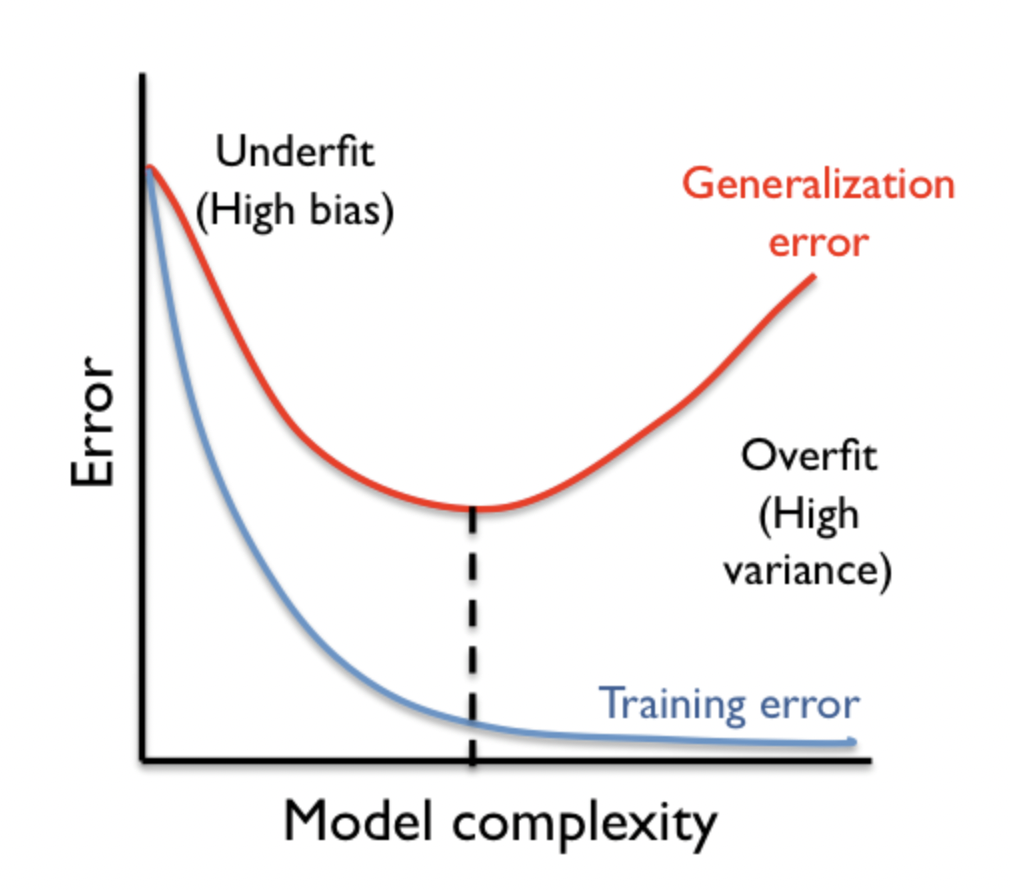
\includegraphics[width=6cm]{images/regularizacao.png}
    \caption{\label{figura1}Conjunto de soluções para o problema.}
  \end{figure}

  % \begin{figure}[H]
  %   \center
  %   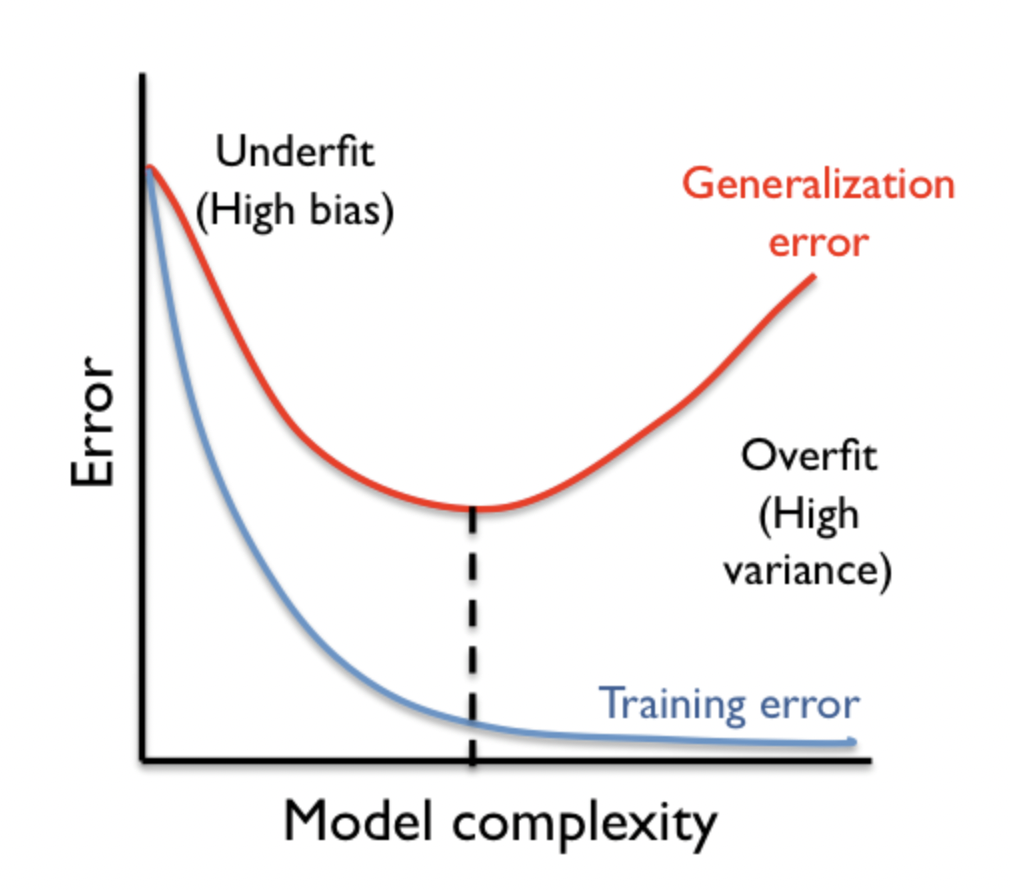
\includegraphics[width=\linewidth]{images/regularizacao.png}
  %   \caption{\label{figura1}Conjunto de soluções para o problema.}
  % \end{figure}